% !TEX root = main.tex

\begin{figure}
% \centering
  \begin{tikzpicture}
    \node[anchor=south west,inner sep=0] (image) at (0,0,0) {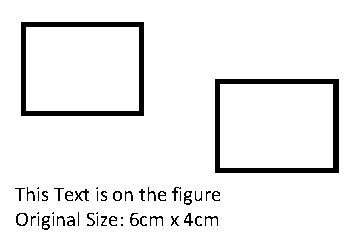
\includegraphics[trim={0 0cm 0 0cm},clip]{../_shared/figure6x4.pdf}};
    \begin{scope}[x={(image.south east)},y={(image.north west)}]
        %% next four lines will help you to locate the point needed by forming a grid.
        %% comment these five lines in the final picture.
        %%%%%% START GRID
        \tikzset{HelpLines/.style={gray!50,line width=0.5pt}};

        \draw[HelpLines,xstep=.1,ystep=.1] (0,0) grid (1,1);
        \draw[HelpLines,xstep=.05,ystep=.05] (0,0) grid (1,1);
        \foreach \x in {0,1,...,9} { \node [anchor=north] at (\x/10,0) {0.\x}; }
        \foreach \y in {0,1,...,9} { \node [anchor=east] at (0,\y/10) {0.\y};}
        %%%%%% END GRID

        \tikzset{LabelStyle/.style={blue,font=\bfseries}};
        \tikzset{BoxStyle/.style={red,line width=1pt}};

        \draw[BoxStyle] (0.5, 0.8) rectangle (0.7, 1.00);

        \draw[dotted,-latex,purple,line width=2pt] (0.7,0.2) -- (0.3, 0.6) node[midway, below]{\ding{192}};

        \node[LabelStyle] at (0.8,0.1) {\ding{202} Annotation};

        % node containing math need to be wrapped
        \begin{scope}[execute at begin node=$, execute at end node=$]
        \node[LabelStyle] at (0.2,0.7) {\sum_{i=0}^\infty \frac{1}{2^n} = 2};
        \end{scope}

    \end{scope}
  \end{tikzpicture}
\caption{Annotated Figure.
The grid is temporary added to the figure to help positioning the annotations.}\label{fig:annotated_figure}
\end{figure}